\section{Introduction}
\subsection{Project Overview}
The purpose of this project is to check that the PCB board of ePATH functions properly. This would help ensure that it was properly manufactured by the factory and it will help smooth identification of faults during maintenance. The process must be automated and user-friendly to enable any technician without good knowledge of the electronics of ePATH perform this test. 

The different components of the testing system and their interactions are briefly induced in Figure \ref{end_goal_diagram}.


\begin{figure}[H]
          \centering
          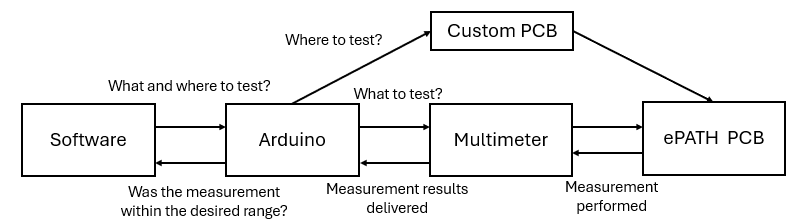
\includegraphics[width=1\linewidth]{img/General end goal diagram.png}
          \caption{Overview of design aspects ePATH testing software.}
          \label{end_goal_diagram}
    \end{figure}

In addition to this some additional small projects were undertaken. Their individual objectives and achievement are described in the Extra projects subsection.

\subsection{Main Objective}
The specific objectives of ePATH Test Bench project were: 
\begin{itemize}
\item To establish computer connection with a multimeter so that measurements from the ePATH PCB can be taken.
\item To design a custom PCB board that selects the appropriate pin from the ePATH PCB to be tested.
\item To develop a GUI that offers an interactive way to do the test.
\item To produce a pdf file with a summary of all the testing results.
\end{itemize}

